\documentclass[a4j]{jarticle}

%% 使用するパッケージ
\usepackage{listings}
\usepackage[]{graphicx}
\usepackage[dvipdfmx]{color}
\usepackage{amssymb}
\usepackage{url}
\西暦

%% 表紙
\title{FAT32解説小冊子}
\author{feynoobs}
\begin{document}

\maketitle

\section{初めに}
本冊子では仮想マシン2台を使用したC言語によるFreeBSDのKernelのデバッグ方法を示す。

なお、UEFIによるBootプログラムとKernelのごく先頭部分はデバッグできない。
UEFIのデバッグはOSDev~\cite{OSDev}を参照されたい。
Kernel先頭部分は机上によるデバッグを行うのみと思われる。

\section{環境準備}
ホストのPCにUbuntu15.10を使用した場合の環境構築手順を示す。
\ref{tb:FreeBSD:_ENV}に示すのアプリケーションがインストール
されていることを前提で話をすすめる。
なおQEMUは``apt-get''コマンドにて``qemu-system-x86''をインストールすると良い。
\begin{table}[htp]
	\caption{必要なアプリケーション}
	\label{tb:FreeBSD:_ENV}
	\centering
	\begin{tabular}{|l|p{10cm}|}									\hline
		アプリケーション	&	概要							\\	\hline	\hline
		QEMU				&	x64エミュレータ				\\	\hline
		OVMF.fd				&	UEFIイメージ					\\	\hline
		FreeBSDイメージ		&	AMD64・UEFI対応のFreeBSDのISO	\\	\hline
	\end{tabular}
\end{table}

\section{環境構築}
\subsection{FreeBSDインストール}
\label{sec:FreeBSD_inst}
\ref{fig:FreeBSD_CREATE}の操作でFreBSDをインストールする仮想ディスクを作成する。
\begin{figure}[htbp]
	\centering
	\begin{lstlisting}[basicstyle=\ttfamily\footnotesize, frame=single, breaklines=true]
$ qemu-img create -f qcow2 GUEST1 16G
	\end{lstlisting}
	\caption{FreeeBSDを格納するファイルシステム作成}
	\label{fig:FreeBSD_CREATE}
\end{figure}

\ref{fig:FreeBSD_QEMU}の操作でFreeBSDをインストール開始する。
\begin{figure}[htbp]
	\centering
	\begin{lstlisting}[basicstyle=\ttfamily\footnotesize, frame=single, breaklines=true]
$ qemu-system-x86_64 -enable-kvm -bios OVMF.fd -hda GUEST1  -cdrom FreeBSD-10.2-RELEASE-amd64-uefi-disc1.iso -m 1024M -smp 2
	\end{lstlisting}
	\caption{FreeBSDをインストールするためのQEMU起動}
	\label{fig:FreeBSD_QEMU}
\end{figure}
QEMUを起動してしばらく経つと\ref{fig:FreeBSD_TOP}の画面になるので
``$<$Install$>$''を選択する。
\begin{figure}[htbp]
	\centering
	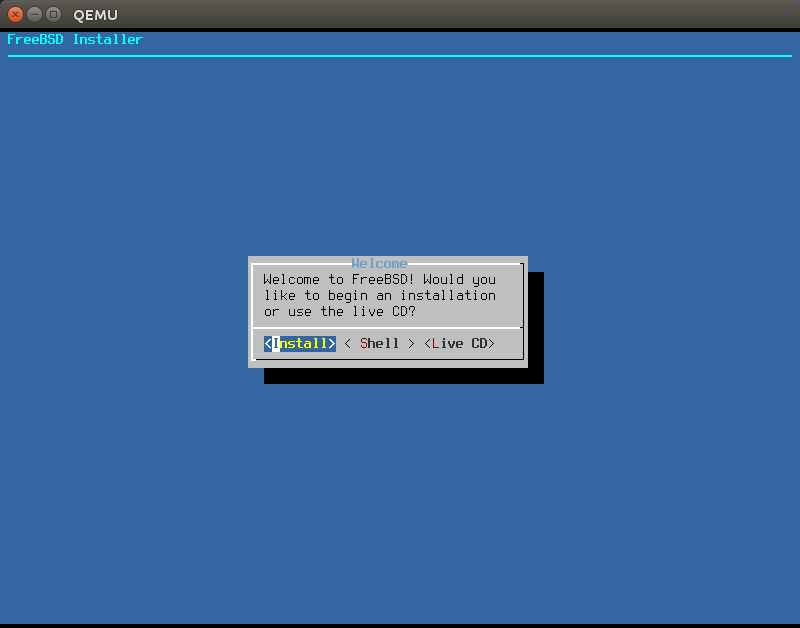
\includegraphics[width=10cm]{./IMG/FreeBSD_TOP.png}
    \caption{インストーラの初期画面}
    \label{fig:FreeBSD_TOP}
\end{figure}

\ref{fig:FreeBSD_KEY}のキーマップ選択画面はPCのキー配置にしたがって選択する。
日本語キーボードの場合は``Japanses 106''で良いであろう。
選択したあと``$>>>$Continue with jp.106.kdb keymap''を選択する。
\begin{figure}[htbp]
	\centering
	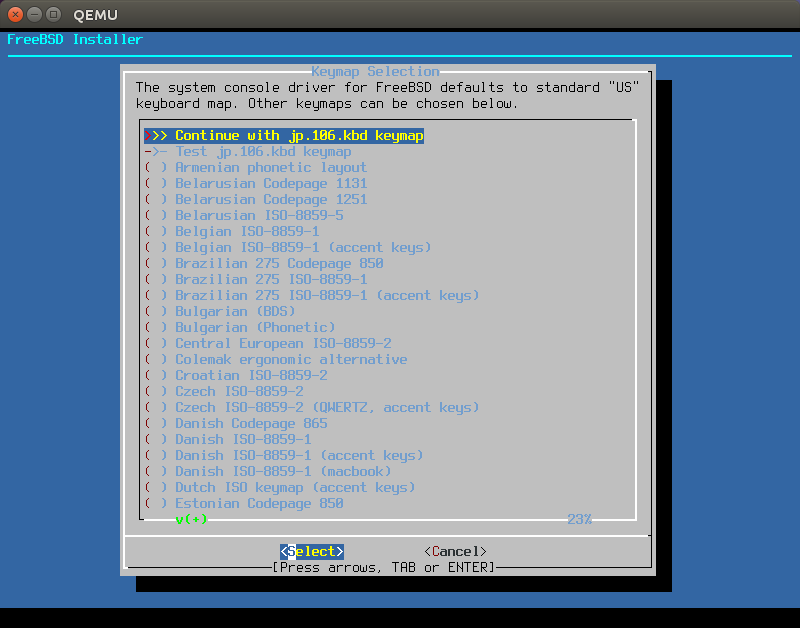
\includegraphics[width=10cm]{./IMG/FreeBSD_JP106.png}
    \caption{キーマップ選択画面}
    \label{fig:FreeBSD_KEY}
\end{figure}

\ref{fig:FreeBSD_HOST}のHOST名は任意の名前でよい。
筆者は``feynoobs''とした。
\begin{figure}[htbp]
	\centering
	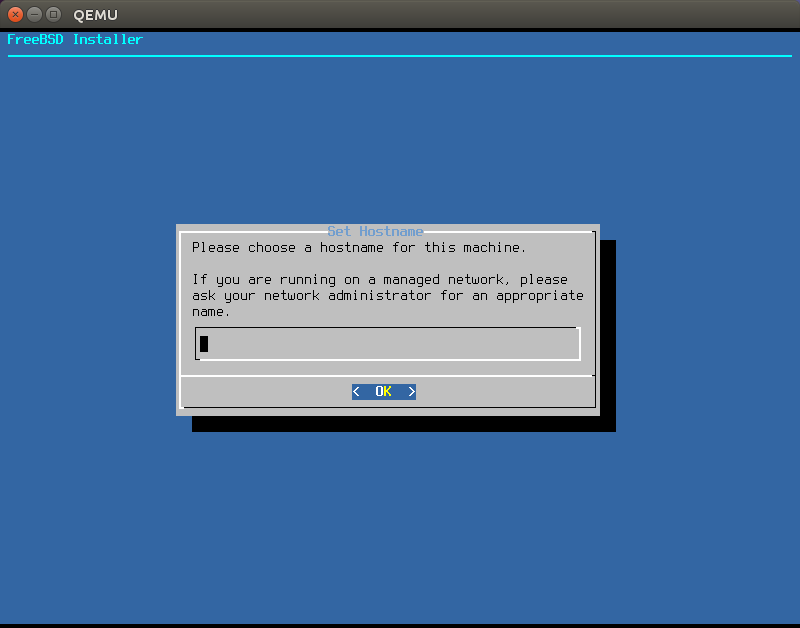
\includegraphics[width=10cm]{./IMG/FreeBSD_HOST.png}
    \caption{ホスト名設定画面}
    \label{fig:FreeBSD_HOST}
\end{figure}

\ref{fig:FreeBSD_INST_SELECT}にて``lib32''と``src''にチェックを入れて確定する。
なお、portsはユーザーとしてFreeBSDを使うときは必須であるが、デバッガとして使う場合は任意である。
\begin{figure}[htbp]
	\centering
	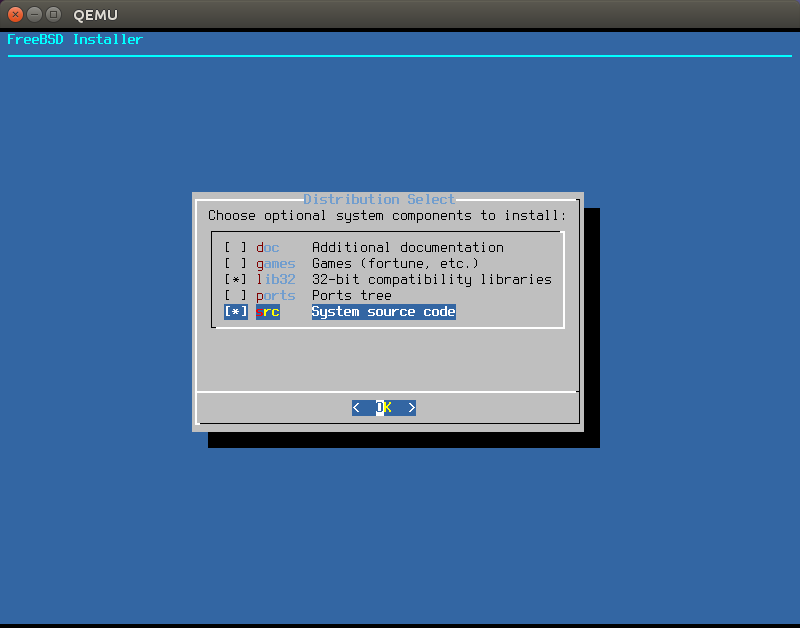
\includegraphics[width=10cm]{./IMG/FreeBSD_INST.png}
    \caption{インストールする対象物}
    \label{fig:FreeBSD_INST_SELECT}
\end{figure}

\ref{fig:FreeBSD_FS}でFreeBSDで使用するファイルシステムを選択する。
通常は``Auto(UFS)''で良い。
\begin{figure}[htbp]
	\centering
	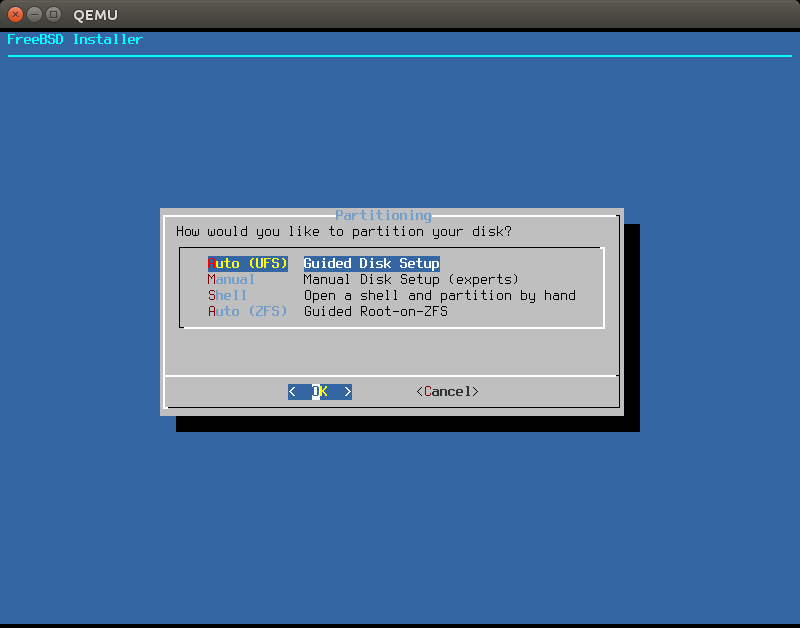
\includegraphics[width=10cm]{./IMG/FreeBSD_AUTO.png}
    \caption{FreeBSDで使用するファイルシステム}
    \label{fig:FreeBSD_FS}
\end{figure}
この仮想マシンにはFreeBSD以外のOSはインストールしないため
\ref{fig:FreeBSD_Q}``$<$Entire Dsik$>$''を選択する。
\begin{figure}[htbp]
	\centering
	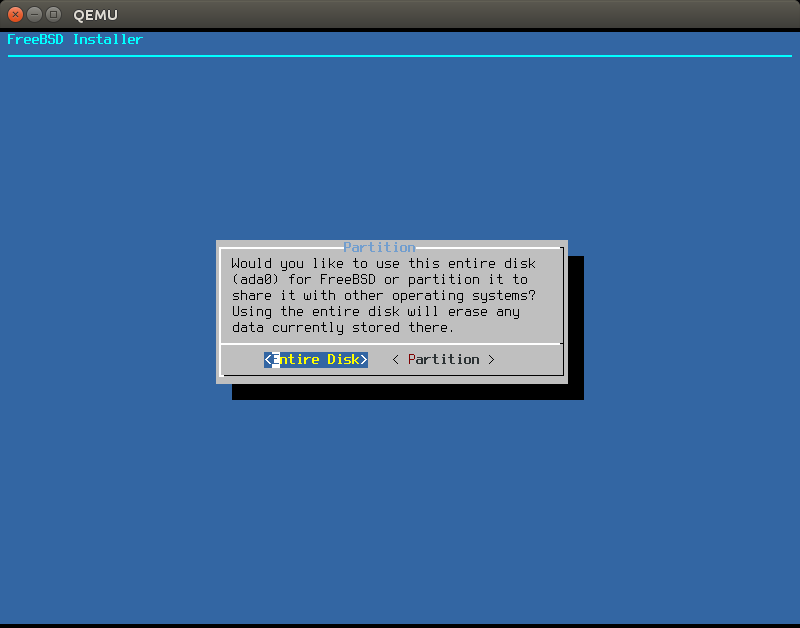
\includegraphics[width=10cm]{./IMG/FreeBSD_ENTRY.png}
    \caption{QEMUでUEFIアプリケーション実行3}
    \label{fig:FreeBSD_Q}
\end{figure}

\ref{fig:FreeBSD_GPT}はストレージ管理を"MBR"で行うか"GPT"で行うかを選択する画面である。
他の管理方法はほとんど使われていないので無視する。
ここではUEFIらしく``MBR''より優れた``GPT''を選択しています。
\begin{figure}[htbp]
	\centering
	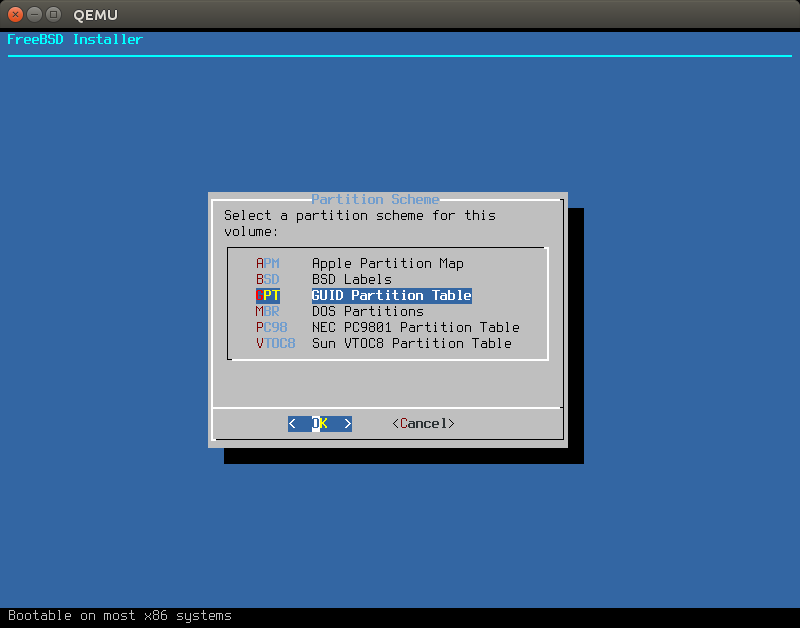
\includegraphics[width=10cm]{./IMG/FreeBSD_GPT.png}
    \caption{ストレージ管理の方式}
    \label{fig:FreeBSD_GPT}
\end{figure}

\ref{fig:FreeBSD_FileSYstem_fin}で``$<$Finish$>$''を選択すると、
\ref{fig:FreeBSD_FileSYstem_com}が表示されるので``$<$Commit$>$''する。
\begin{figure}[htbp]
	\centering
	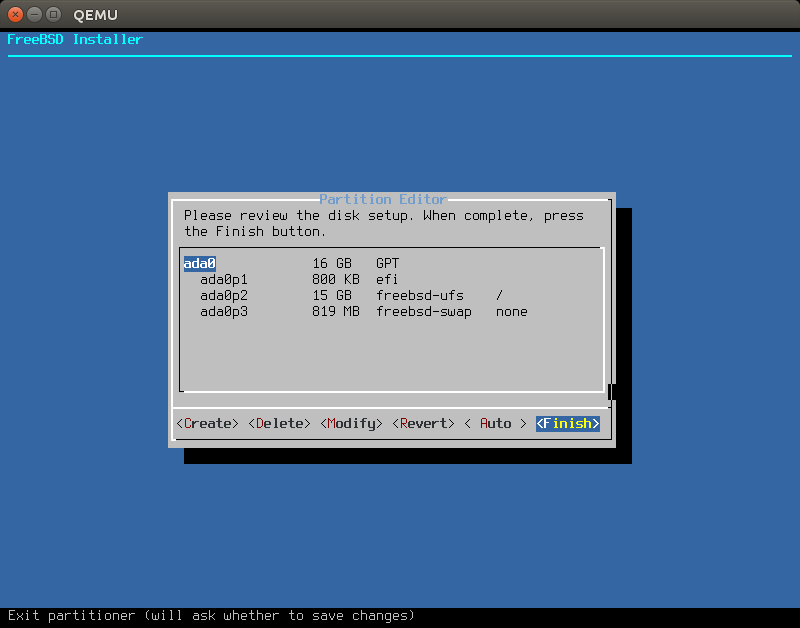
\includegraphics[width=10cm]{./IMG/FreeBSD_PT_FIX.png}
    \caption{ファイルシステム確定}
    \label{fig:FreeBSD_FileSYstem_fin}
\end{figure}
\begin{figure}[htbp]
	\centering
	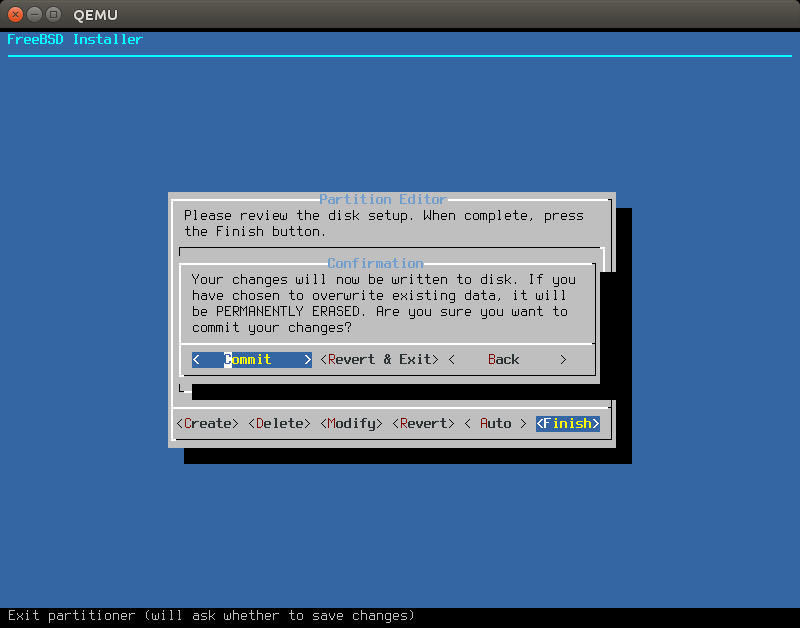
\includegraphics[width=10cm]{./IMG/FreeBSD_COMMIT.png}
    \caption{ファイルシステムコミット}
    \label{fig:FreeBSD_FileSYstem_com}
\end{figure}

インストール作業が終わると\ref{fig:FreeBSD_PASS}の画面でrootのパスワードを設定する。
パスワードを設定したくない場合はそのままエンターキーを押下する。
\begin{figure}[htbp]
	\centering
	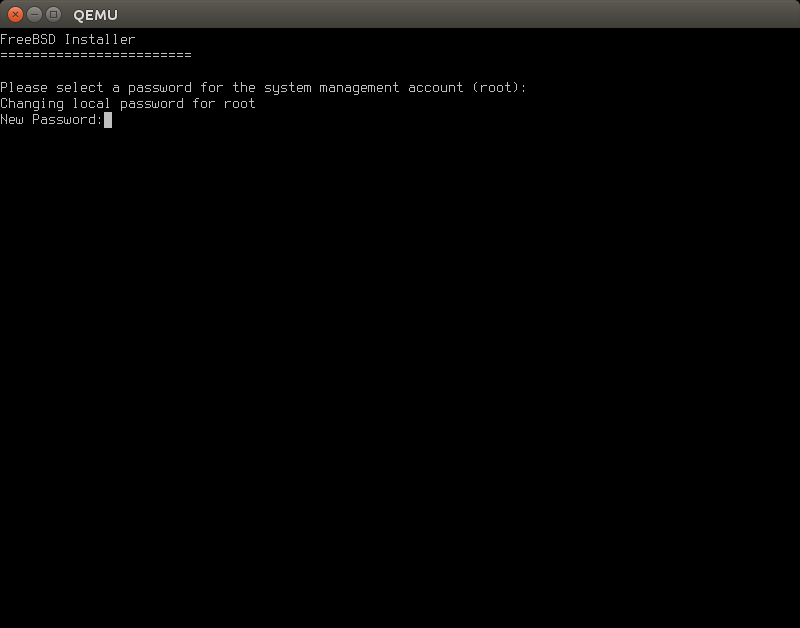
\includegraphics[width=10cm]{./IMG/FreeBSD_ROOT_PASS.png}
    \caption{パスワード設定画面}
    \label{fig:FreeBSD_PASS}
\end{figure}

続いて\ref{fig:FreeBSD_NIC}のようなNIC設定の画面が表示される。
筆者は設定なかったので``$<$Cancel$>$''を選択した。
ネットワークの設定は割愛する。
\begin{figure}[htbp]
	\centering
	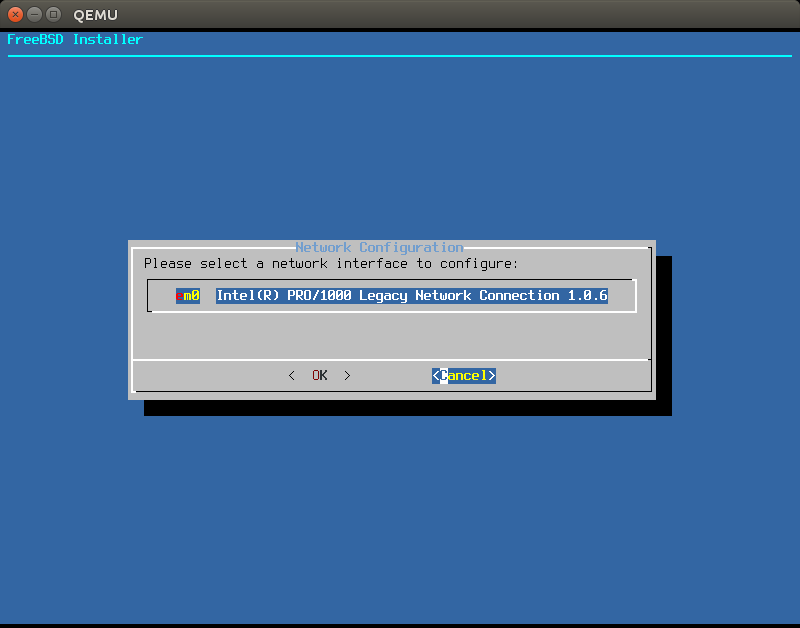
\includegraphics[width=10cm]{./IMG/FreeBSD_NIC.png}
    \caption{NIC設定画面}
    \label{fig:FreeBSD_NIC}
\end{figure}

次にタイムゾーンの設定を行う。
\ref{fig:FreeBSD_TIM}にて``$<$No$>$''を選択後、
\ref{fig:FreeBSD_TIM2}の国を選ぶリストで``18 Japan''を選択する。
\begin{figure}[htbp]
	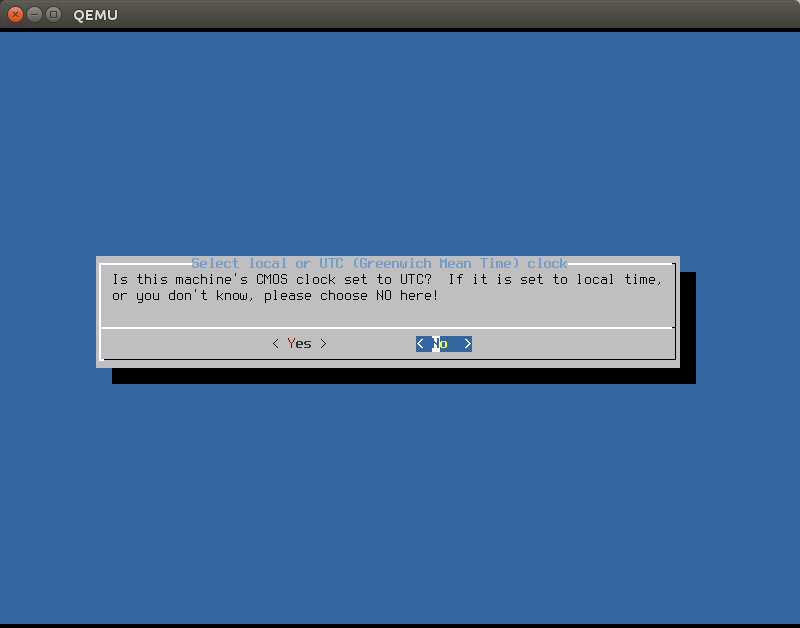
\includegraphics[width=10cm]{./IMG/FreeBSD_TIM.png}
	\centering
    \caption{タイムゾーン設定1}
    \label{fig:FreeBSD_TIM}
\end{figure}
\begin{figure}[htbp]
	\centering
	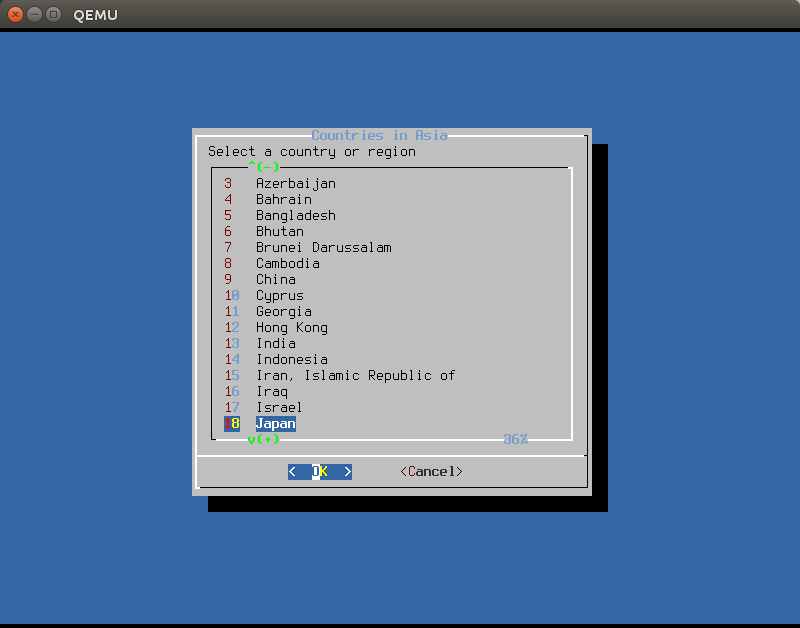
\includegraphics[width=10cm]{./IMG/FreeBSD_TIM_JP.png}
    \caption{タイムゾーン設定2}
	\label{fig:FreeBSD_TIM2}
\end{figure}

\ref{fig:FreeBSD_Service}で有効にするサービスを選ぶ。
筆者はsshdを無効にしているが、特に初期値でも問題ない。
\begin{figure}[htbp]
	\centering
	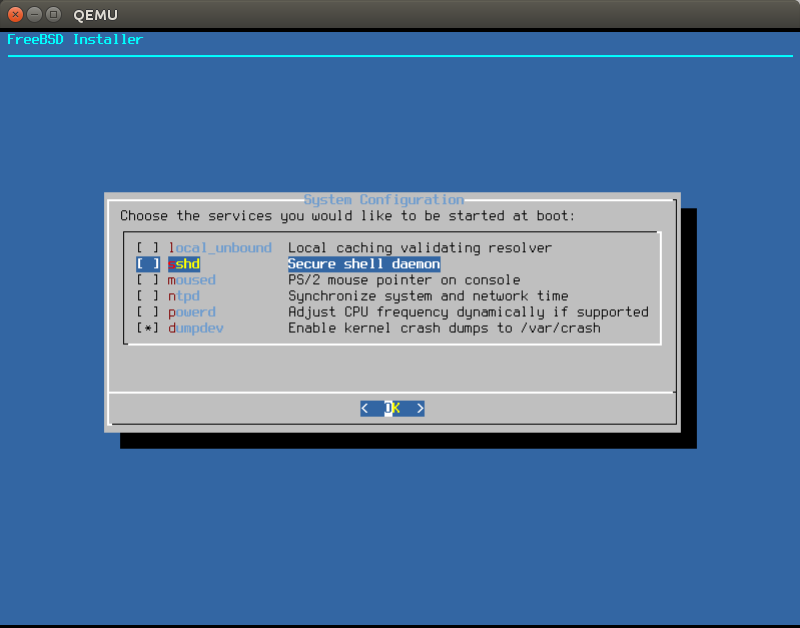
\includegraphics[width=10cm]{./IMG/FreeBSD_SYS.png}
    \caption{FreeBSDで実行するサービス}
    \label{fig:FreeBSD_Service}
\end{figure}

\ref{fig:FreeBSD_ADD_U}にて一般ユーザの追加えるが、
デバッガで一般ユーザをいれる理由もないので筆者は``$<$No$>$''を選択した。
\begin{figure}[htbp]
	\centering
	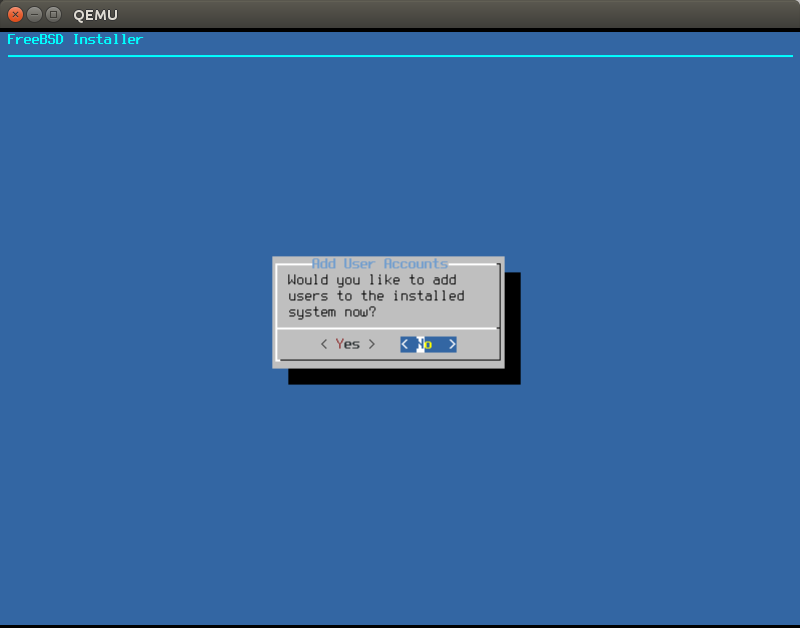
\includegraphics[width=10cm]{./IMG/FreeBSD_ADD_USER.png}
    \caption{一般ユーザ追加}
    \label{fig:FreeBSD_ADD_U}
\end{figure}
\clearpage

以降はインストールの完了作業である。
\ref{fig:FreeBSD_FIN_1}にて``Exit''を選択し、
\ref{fig:FreeBSD_FIN_2}にて``$<$No$>$''を選択し、
\ref{fig:FreeBSD_FIN_3}にて``$<$Reboot$>$''を選択すれば
インストールが完了してリブートする。
リブートが完了したら、一旦QEMUを終了させる。
\begin{figure}[htbp]
	\centering
	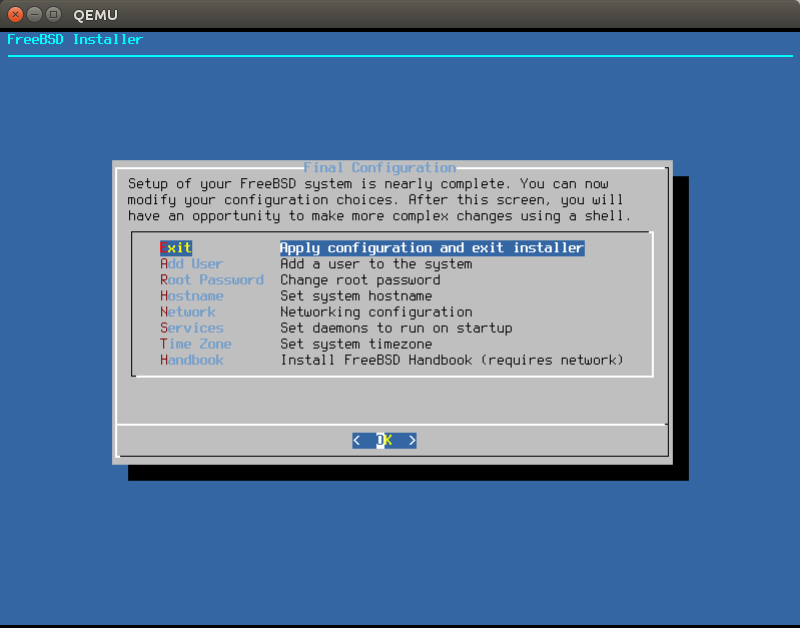
\includegraphics[width=10cm]{./IMG/FreeBSD_FIN.png}
    \caption{FreeBSDインストール完了1}
    \label{fig:FreeBSD_FIN_1}
\end{figure}
\begin{figure}[htbp]
	\centering
	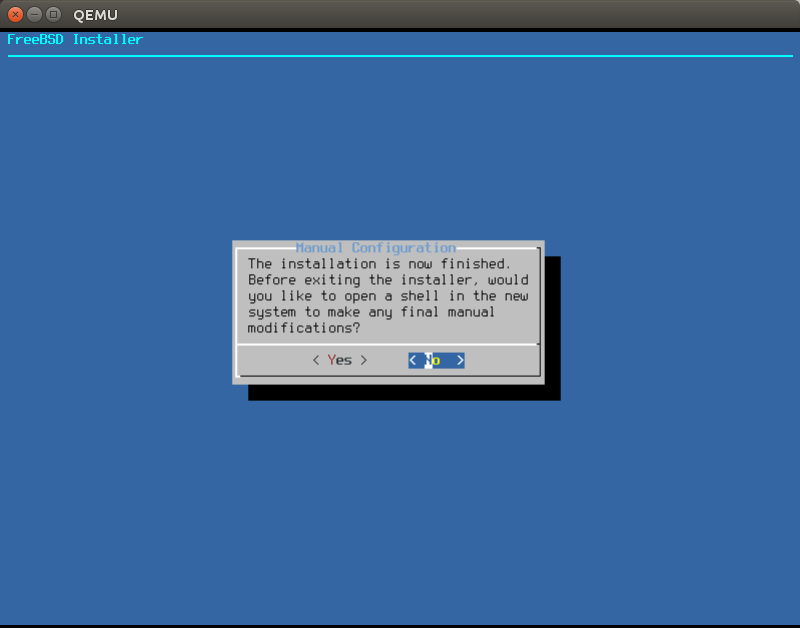
\includegraphics[width=10cm]{./IMG/FreeBSD_LST.png}
    \caption{FreeBSDインストール完了2}
    \label{fig:FreeBSD_FIN_2}
\end{figure}
\begin{figure}[htbp]
	\centering
	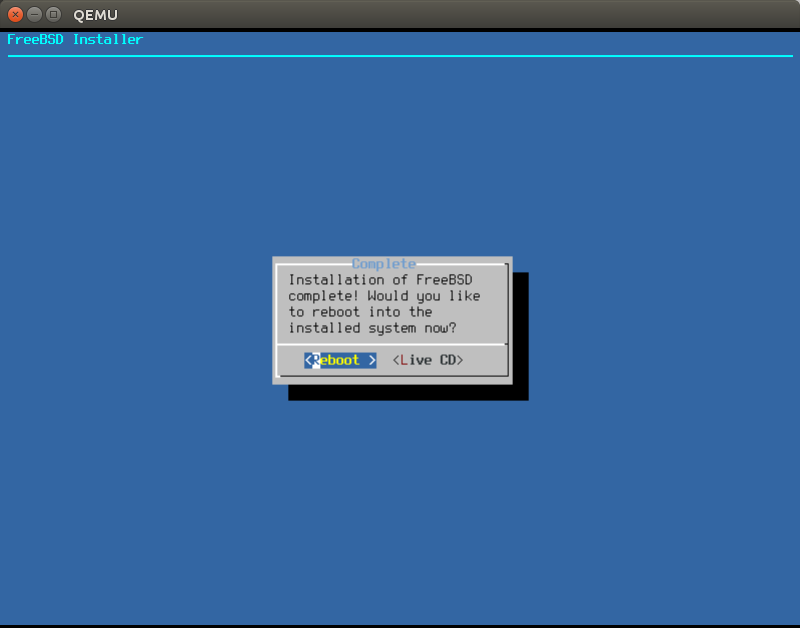
\includegraphics[width=10cm]{./IMG/FreeBSD_ALL_LAS.png}
    \caption{FreeBSDインストール完了3}
    \label{fig:FreeBSD_FIN_3}
\end{figure}


\subsection{Kernelの再構築のためのファイル編集}
\ref{sec:FreeBSD_inst}でインストールしたFreeBSDをデバッグできるようにKernelを再構築する。

\ref{fig:FreeBSD_boot_com}のコマンドでQEMUを起動する。
\begin{figure}[htbp]
	\centering
	\begin{lstlisting}[basicstyle=\ttfamily\footnotesize, frame=single, breaklines=true]
$ qemu-system-x86_64 -enable-kvm -bios OVMF.fd -hda GUEST1 -m 1024M -smp 2
    \end{lstlisting}
	\caption{FreeeBSDを仮想ストレージから起動}
	\label{fig:FreeBSD_boot_com}
\end{figure}

インストールできている場合は、しばらく経つと\ref{fig:FreeBSD_BOOT}の画面になる。
\begin{figure}[htbp]
	\centering
	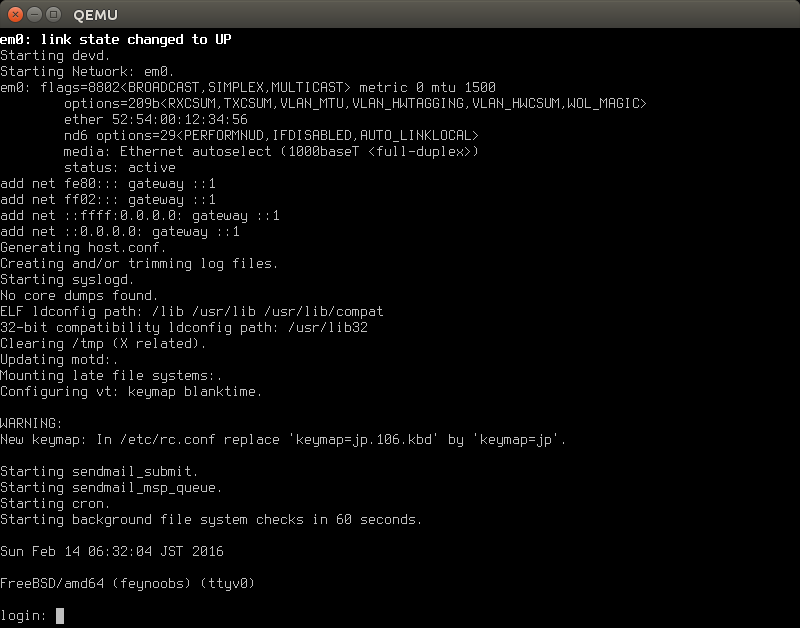
\includegraphics[width=10cm]{./IMG/FreeBSD_BOOT.png}
    \caption{FreeBSD起動画面}
    \label{fig:FreeBSD_BOOT}
\end{figure}

ログイン後3つのファイルを編集する。
なおFreeBSDインストール完了時には``vi''と``ee''の2つのエディタが組み込まれている。
筆者のように``vi''が苦手な者は、``ee''が直感的に使いやすいとであろう。
\begin{itemize}
    \item /boot/device.hints
    \item /sys/amd64/conf/GENERIC.hints
    \item /sys/amd64/conf/GENERIC
\end{itemize}

\subsubsection{device.hintsの編集}
\label{sec:FreeBSD_device.hints}
device.hintsの中に\ref{fig:FreeBSD_bf_hints}の行がある。
この行を\ref{fig:FreeBSD_af_hints}に書き換えてエディタを閉じる。
\begin{figure}[htbp]
	\centering
	\begin{lstlisting}[basicstyle=\ttfamily\footnotesize, frame=single, breaklines=true]
hint.uart.0.flags="0x10"
	\end{lstlisting}
	\caption{hints編集前}
	\label{fig:FreeBSD_bf_hints}
\end{figure}

\begin{figure}[htbp]
	\centering
	\begin{lstlisting}[basicstyle=\ttfamily\footnotesize, frame=single, breaklines=true]
hint.uart.0.flags="0x90"
	\end{lstlisting}
	\caption{hints編集後}
	\label{fig:FreeBSD_af_hints}
\end{figure}

\subsubsection{GENERIC.hintsの編集}
device.hintsと全く同じなので割愛する。

\subsubsection{GENERICの編集}
GENERICの適当な場所に\ref{fig:FreeBSD_GENERIC}の内容を追記する。
\begin{figure}[htbp]
	\centering
	\begin{lstlisting}[basicstyle=\ttfamily\footnotesize, frame=single, breaklines=true]
options     DDB
options     GDB
	\end{lstlisting}
	\caption{GENERICの編集}
	\label{fig:FreeBSD_GENERIC}
\end{figure}

\subsection{Kernelの再構築実行}
\label{sec:Kern_build}
``/sys/amd64/conf''にて\ref{fig:FreeBSD_cf}を実行する。
そうすると、``/sys/amd64/compile/GENERIC''配下にKernelのソースコードが生成される。
これをコンパイルすることで新しいデバッグ用のKernelを作ることができる。
\begin{figure}[htbp]
	\centering
	\begin{lstlisting}[basicstyle=\ttfamily\footnotesize, frame=single, breaklines=true]
$ config GENERIC
	\end{lstlisting}
	\caption{configファイルコンパイル}
	\label{fig:FreeBSD_cf}
\end{figure}

コンパイルは\ref{fig:FreeBSD_kern}で実行する。
エラーなく終わればデバッグ用Kernelが生成されインストールされている。
ここまでで、一度シャットダウンする。
\begin{figure}[htbp]
	\centering
	\begin{lstlisting}[basicstyle=\ttfamily\footnotesize, frame=single, breaklines=true]
$ make cleandepend && make depend && make && make install
	\end{lstlisting}
	\caption{Kernelコンパイル}
	\label{fig:FreeBSD_kern}
\end{figure}

\section{Kernelデバッグ開始}
\subsection{Kernelイメージの複製とパイプ生成}
\ref{fig:FreeBSD_CREATE}で作成したストレージのイメージをコピーする。
GUEST1をGUEST2とORGにコピーしたとして話を進める。
なお、ORGはストレージイメージが壊れた時のバックアップ用である。
実際、FreeBSDをシャットダウンせずにQEMUを終了すると、次回起動できなくなる場合があった。

次に仮想マシン2つをつなぐパイプの作成を行うため
\ref{fig:FreeBSD_pipe}を実行する。
\begin{figure}[htbp]
	\centering
	\begin{lstlisting}[basicstyle=\ttfamily\footnotesize, frame=single, breaklines=true]
$ mkfifo /tmp/fifoA.in /tmp/fifoA.out
$ ln -s /tmp/fifoA.out /tmp/fifoB.in
$ ln -s /tmp/fifoA.in /tmp/fifoB.out
	\end{lstlisting}
	\caption{仮想マシンを接続するパイプ作成}
	\label{fig:FreeBSD_pipe}
\end{figure}

\subsection{GUEST1設定}
\ref{fig:FreeBSD_guest1}のようにしてGUEST1を起動する。
\begin{figure}[htbp]
	\centering
	\begin{lstlisting}[basicstyle=\ttfamily\footnotesize, frame=single, breaklines=true]
$ qemu-system-x86_64 -enable-kvm -hda GUEST1 -bios OVMF.fd -m 1024M -smp 2 -serial pipe:/tmp/fifoA
	\end{lstlisting}
	\caption{GUEST1起動1}
	\label{fig:FreeBSD_guest1}
\end{figure}

起動して\ref{fig:FreeBSD_CNTDN}のように、ブートへのカウントダウンが始まると
エンター以外の例えばスペースなどのキーを押下する。
そうすると``OK''と表示されたプロンプト(OKプロンプト)が表示される。

ここに\ref{fig:FreeBSD_OK}のように``boot -dg''とタイプしてエンターキーを押下する。
\begin{figure}[htbp]
	\centering
	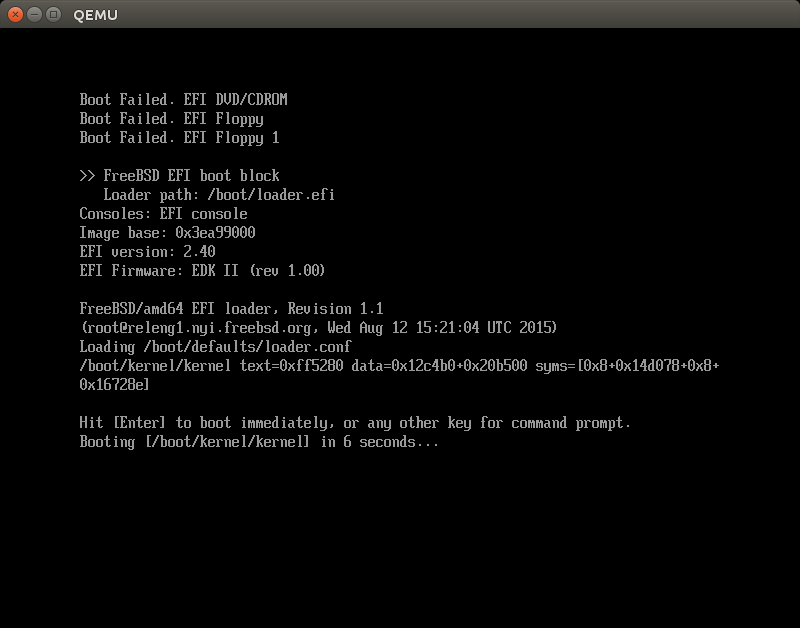
\includegraphics[width=10cm]{./IMG/FreeBSD_CNTDN.png}
    \caption{起動カウントダウン}
    \label{fig:FreeBSD_CNTDN}
\end{figure}
\begin{figure}[htbp]
	\centering
	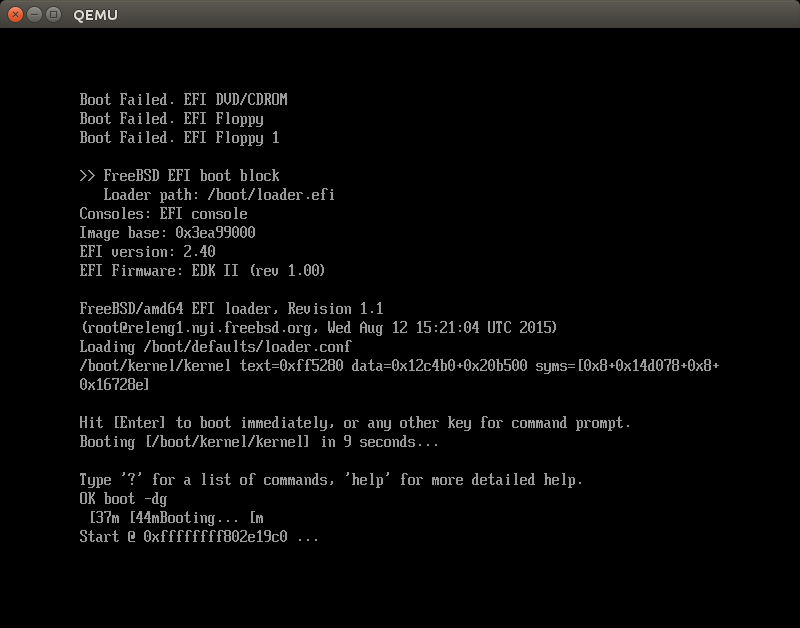
\includegraphics[width=10cm]{./IMG/FreeBSD_OK.png}
    \caption{OKプロンプトでの入力}
    \label{fig:FreeBSD_OK}
\end{figure}
少し文字が出たあと止まってしまうが正常である。
以上でGUEST1の設定は終了する。

\subsection{GUEST2設定}
\ref{fig:FreeBSD_guest2}のようにしてGUEST2を起動する。
\begin{figure}[htbp]
	\centering
	\begin{lstlisting}[basicstyle=\ttfamily\footnotesize, frame=single, breaklines=true]
$ qemu-system-x86_64 -enable-kvm -hda GUEST2 -bios OVMF.fd -m 1024M -smp 2 -serial pipe:/tmp/fifoB
	\end{lstlisting}
	\caption{GUEST2起動}
	\label{fig:FreeBSD_guest2}
\end{figure}

こちらは通常に起動させる。
そうして\ref{sec:Kern_build}でKernelをコンパイルしたパス(``/sys/amd64/compile/GENERIC'')に移動する。
このパスで\ref{fig:FreeBSD_gdb}のように入力する。
\begin{figure}[htbp]
	\centering
	\begin{lstlisting}[basicstyle=\ttfamily\footnotesize, frame=single, breaklines=true]
$ kgdb kernel.debug
	\end{lstlisting}
	\caption{Kernelデバッガ起動}
	\label{fig:FreeBSD_gdb}
\end{figure}

KGDが起動するので最初に\ref{fig:FreeBSD_gdb_cuau0}と入力する。
以上でGUEST1とGUEST2が接続され、KGDBによるデバッグが可能になる。
\begin{figure}[htbp]
	\centering
	\begin{lstlisting}[basicstyle=\ttfamily\footnotesize, frame=single, breaklines=true]
$ (kgdb) target remote /dev/cuau0
	\end{lstlisting}
	\caption{GUEST1とGUEST2の接続}
	\label{fig:FreeBSD_gdb_cuau0}
\end{figure}

\section{Kernelデバッグのテクニック}
\subsection{CPUレジスタを確認する}
Kernelデバッグ時にCPUレジスタの中身を確認したくなるシーンは多々あるが、
KGDBではすべてのレジスタは見れない。
そこでQEMUから見る方法を紹介する。
\ref{fig:FreeBSD_guest1}を\ref{fig:FreeBSD_guest1_reg}に書き換えること。
\begin{figure}[htbp]
	\centering
		\begin{lstlisting}[basicstyle=\ttfamily\footnotesize, frame=single, breaklines=true]
$ qemu-system-x86_64 -enable-kvm -hda GUEST1 -bios OVMF.fd -m 1024M -smp 2 -serial pipe:/tmp/fifoA -monitor stdio
		\end{lstlisting}
	\caption{GUEST1起動2}
	\label{fig:FreeBSD_guest1_reg}
\end{figure}
そして、QEMUを起動したターミナルから\ref{fig:QEMU_reg_chk}と入力する。
\begin{figure}[htbp]
	\centering
	\begin{lstlisting}[basicstyle=\ttfamily\footnotesize, frame=single, breaklines=true]
(qemu) info registers
	\end{lstlisting}
	\caption{(QEMU)プロンプトでの入力}
	\label{fig:QEMU_reg_chk}
\end{figure}

\ref{fig:QEMU_REG_INFO}のようにレジスタ一覧が出れば成功である。
\begin{figure}[htbp]
	\centering
    	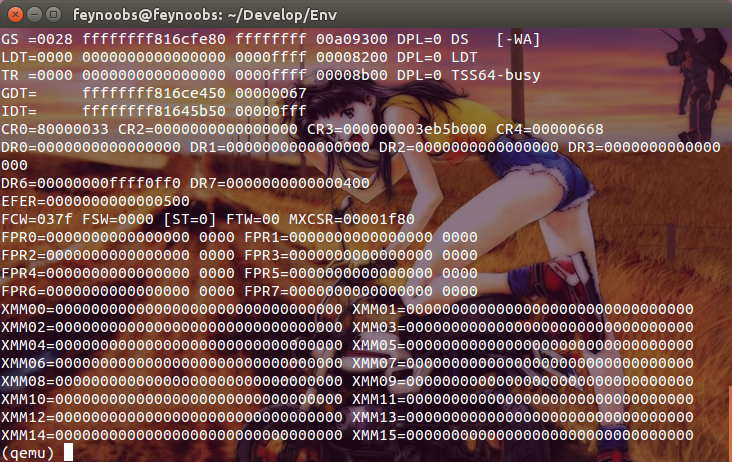
\includegraphics[width=10cm]{./IMG/QEMU_INFO_REGISTERS.png}
    \caption{レジスタ一覧の例}
    \label{fig:QEMU_REG_INFO}
\end{figure}

\section{終わりに}
本小冊子ではKGDBを用いたFreeBSD Kernelのデバッグの入り口を
インストールから示した。
KGDBは2台のマシンが必要であり、手順がわずらわしいがC言語で
Kernelのデバッグが行えるのが魅力である。

その他DDBを使用すれば1台のマシンでデバッグ可能であるが、
アセンブリでのデバッグになるため説明は行わなかった。
興味のある者はWebなどで情報を探して実行して欲しい。

\begin{thebibliography}{9}
	\bibitem{OSDev}	OSDev \url{http://wiki.osdev.org/Debugging_UEFI_applications_with_GDB}
\end{thebibliography}

\end{document}
